\documentclass{article}
\usepackage{graphicx}
\usepackage{amsmath}
\usepackage{pgfplots}
\usepackage{physics}
\usepackage{cancel}
\usepackage{enumitem}
\usepackage{txfonts}
\usepackage[normalem]{ulem}

\newcommand{\g}{\text{g}}
\newcommand{\kilo}{\text{k}}
\newcommand{\m}{\text{m}}
\newcommand{\centi}{\text{c}}
\newcommand{\s}{\text{s}}
\newcommand{\N}{\text{N}}
\newcommand{\J}{\text{J}}
\newcommand{\C}{\text{C}}
\newcommand{\V}{\text{V}}
\newcommand{\A}{\text{A}}
\newcommand{\Ohm}{\text{\Omega}}

\pgfplotsset{compat=1.18}

\pgfplotsset{compat=1.18}

\usepackage[a4paper, top=1cm, bottom=2cm, left=2cm, right=2cm, includehead, includefoot]{geometry}



\begin{document}

\noindent
Physics 4B - Electromagnetism \hfill Prof. Alfred Cauthen
\noindent\rule{\textwidth}{0.4pt}

\begin{center}
    \textbf{\LARGE Homework 2} \\
    \vspace{12pt}
    \large Aaron W. Tarajos \\
    \textit{\today}
\end{center}

\noindent\rule{\textwidth}{0.4pt}

\section*{Chapter 21 Problem 52}
A particle of charge $Q$ is fixed at the origin of an $xy$ coordinate system. 
At t = 0 a particle ($m$ = 0.800 g, $q$ = 4.00 $\mu$C) is located on the $x$ axis at $x$ = 20.0 cm, moving with a speed of 50.0 m/s in the positive $y$ direction. 
For what value of $Q$ will the moving particle execute circular motion? (Neglect the gravitational force on the particle.)

\subsection*{Solution}
We can solve for $Q$ using the relationship between centripetal force and tangential velocity.
\begin{align*}
	F_c &= m a_c \\
	k \frac{Qq}{r^2} &= m \omega^2 r \\
	k \frac{Qq}{r^2} &= m \frac{v_t^2}{r} \\
	Q &= m \frac{v_t^2 r}{qk}
\end{align*}
then we substitute the known variables;
\[
	Q = 0.800\ \g \frac{\left( 50\ \m / \s \right)^2 20.0\ \centi \m}{4.00\ \mu \C \cdot 8.99 \times 10^9\ \N \cdot \frac{\m^2}{\C^2}} = \boxed{0.111 \times 10^{-4}\ \C}	
\]

\section*{Chapter 21 Problem 66}
An electron is in a vacuum near Earth’s surface and located at $y$ = 0 on a vertical $y$ axis. 
At what value of $y$ should a second electron be placed such that its electrostatic force on the first electron balances the gravitational force on the first electron?

\subsection*{Solution}
I am going to assume that it is okay to ignore the gravitational effects of the two electrons on eachother, in which case we just need set the gravitational force equal to the electrostatic force and solve for $r$.
\begin{align*}
	F_g &= k\frac{e^2}{r^2} \\
	r^2 &= k\frac{e^2}{F_g} \\
	r &= \sqrt{k \frac{e^2}{F_g}}
\end{align*}
and now we solve for $r$ using the known variables
\[
	r = \sqrt{8.99 \times 10^9\ \N \cdot \frac{\m^2}{\C^2} \frac{(1.602 \times 10^{-19}\ \C)^2}{9.109 \times 10^{-31}\ \kilo\g \cdot 9.81\ \frac{\m}{\s^2}}} = \boxed{5.081\ \m} 
\]

\section*{Chapter 22 Question 4}
Figure 22-25 shows four situations in which four charged particles are evenly spaced to the left and right of a central point. 
The charge values are indicated. 
Rank the situations according to the magnitude of the net electric field at the central point, greatest first.

\begin{figure}[ht]
    \centering
    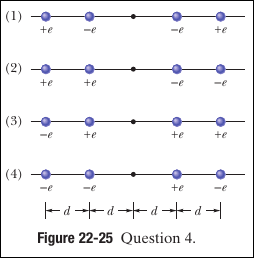
\includegraphics[scale=0.75]{image-1.png}
\end{figure}

\subsection*{Solution}
First we will intuitively explain the solution and then prove it. 
For set (1), the net charge will be zero because for a test charge placed that the origin, the field created by a particle on the given side is exactly equal to the field created in the opposite direction by the symmetrical particle on the other side.
Set (2) we expect to have the highest magnitude for a reason that is sort of the inverse of set (1). For each of the two particles on one side, there is a particle off opposite charge at the same distance on the other side effectively doubling the magnitude of the electric field.
Then we expect set (4) to have a greater field magnitude than set (3) because the closer particles generate a higher field strength than the further ones and we can see the positioning of the non-symmetrical charges are further in (3) than in (4).
So we have;
\[
	\boxed{2 > 4 > 3 > 1}
\]

\subsubsection*{Proof}
\begin{align*}
	\vec{E}_1 &= k\left( \frac{e}{d^2} + \frac{e}{4d^2} - \frac{e}{d^2} - \frac{e}{4d^2} \right) = k (0) = 0 \\
	\vec{E}_2 &= k\left( \frac{e}{d^2} + \frac{e}{4d^2} + \frac{e}{d^2} + \frac{e}{4d^2} \right) = k \left( \frac{5e}{2d^2} \right) \\
	\vec{E}_3 &= k\left( \frac{e}{d^2} + \frac{e}{4d^2} - \frac{e}{d^2} + \frac{e}{4d^2} \right) = k \left( \frac{e}{2d^2} \right) \\
	\vec{E}_4 &= k\left( \frac{e}{d^2} + \frac{e}{4d^2} + \frac{e}{d^2} - \frac{e}{4d^2} \right) = k \left( \frac{2e}{d^2} \right) \\
\end{align*}
\[
	k \left( \frac{5e}{2d^2} \right) > k \left( \frac{2e}{d^2} \right) > k \left( \frac{e}{2d^2} \right) > 0	
\]

\section*{Chapter 22 Question 5}
Figure 22-26 shows two charged particles fixed in place on an axis. (a) Where on the axis (other than at an infinite distance) is there a point at which their net electric field is zero: between the charges, to their left, or to their right? 
(b) Is there a point of zero net electric field anywhere off the axis (other than at an infinite distance)?

\begin{figure}[ht]
    \centering
    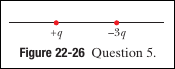
\includegraphics[scale=0.75]{image-2.png}
\end{figure}

\subsection*{Solution}
Let the origin be located at $+q$, then we write the net electric field at point $x$ as the sum of these values and we want to find where it equals zero.
\begin{align*}
	\vec{E} = k\left( \frac{q}{x^2} + \frac{-3q}{\left(d-x\right)^2} \right) \\
	0 = \frac{q}{x^2} - \frac{3q}{\left(d-x\right)^2} \\
	\frac{q}{x^2} = \frac{3q}{\left(d-x\right)^2} \\
	\left(d-x\right)^2 = 3x^2 \\
	d-x = - \sqrt{3}x \\
	\boxed{x = \frac{d}{1-\sqrt{3}}}
\end{align*}
We only consider the negative root because if a positive test charge was on the right of $+q$ then the field from both particles would be in the same direction and could not sum to zero.
Now for the second part; there is no point off the axis, other than infinitely far, with zero net electric field. \\
\textbf{Proof:} The respective $x$ and $y$ components of our field vector must sum to zero. Starting with the $y$ component
\begin{align*}
	\frac{y}{r_1^3} &= 3\frac{y}{r_2^3} \\
	\frac{1}{r_1^3} &= \frac{3}{r_2^3} \\
	r_2^3 &= 3r_1^3 \\
	r_2 &= \sqrt[3]{3} r_1
\end{align*}
which we can substitute into the $x$ component equations
\begin{align*}
	\frac{x}{r_1^3} &= 3 \frac{x-d}{r_d^3} \\
	\frac{x}{r_1^3} &= 3 \frac{x-d}{\left(\sqrt[3]{3} r_1\right)^3} \\
	\frac{x}{r_1^3} &= 3 \frac{x-d}{3 r_1^3} \\
	x = x-d
\end{align*}
which is only a valid statement for $d=0$. Therefore there is no point off axis that $E = 0$.

\section*{Chapter 22 Problem 8}
In Fig. 22-36, the four particles are fixed in place and have charges $q_1 = q_2 = +5e$, $q_3 = +3e$, and $q_4 = -12e$.
Distance $d = 5.0$ $\mu$m. What is the magnitude of the net electric field at point $P$ due to the particles?

\begin{figure}[ht]
    \centering
    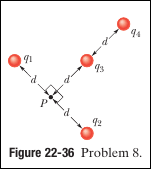
\includegraphics[scale=0.75]{image-3.png}
\end{figure}

\subsection*{Solution}
We can ignore the effects of $q_1$ and $q_2$, because of the symmetry, therefore we have;
\begin{align*}
	\vec{E}_P &= k\left(\frac{q_3}{d^2} + \frac{q_4}{d^2}\right) \\
			  &= 8.99 \times 10^9\ \N \cdot \frac{\m^2}{\C^2} \left( \frac{3 \cdot 1.602 \times 10^{-19}\ \C}{5.0^2\ \mu^2 \m^2} + \frac{-12 \cdot 1.602 \times 10^{-19}\ \C}{4 \cdot 5.00^2\ \mu^2\m^2}\right) \\
			  &= \boxed{0\ \frac{\N}{\C}}
\end{align*}

\section*{Chapter 22 Problem 12}
Figure 22-39 shows an uneven arrangement of electrons (e) and protons (p) on a circular arc of radius $r = 2.00$ cm, with angles $\theta_1 = 30.0^\circ$, $\theta_2 = 50.0^\circ$, $\theta_3 = 30.0^\circ$, and $\theta_4 = 20.0^\circ$. 
What are the (a) magnitude and (b) direction (relative to the positive direction of the x-axis) of the net electric field produced at the center of the arc?

\begin{figure}[ht]
    \centering
    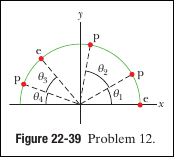
\includegraphics[scale=0.75]{image-4.png}
\end{figure}

\subsection*{Solution}
The charge positions and their respective angles are:

\[
    \begin{aligned}
        q_1 &= -e \quad (\theta_0 = 0^\circ)     && \text{(electron at +x axis)} \\
        q_2 &= +e \quad (\theta_1 = 30^\circ)    && \text{(proton)} \\
        q_3 &= +e \quad (\theta_2 = 50^\circ)    && \text{(proton)} \\
        q_4 &= -e \quad (\theta_3 = 20^\circ)   && \text{(electron)} \\
        q_5 &= +e \quad (\theta_4 = 20^\circ)   && \text{(proton)}
    \end{aligned}
\]
Each charge contributes an electric field at the center with components:

\[
    E_{x} = k\,\frac{e}{r^{2}}\Bigl[\cos0 
                                - \cos30
                                - \cos80
                                - \cos130
                                + \cos160 \Bigr],
\]

\[
    E_{y} = k\,\frac{e}{r^{2}}\Bigl[\sin0 
                                - \sin30
                                - \sin80
                                + \sin200
                                - \sin230 \Bigr].
\]
Substituting the values:

\begin{align*}
	E_{x} &= (8.99 \times 10^9) \frac{(1.60 \times 10^{-19})}{(0.020)^2}
    \Bigl[1 - 0.866 - 0.174 - (-0.643) + (-0.940)\Bigr], \\
	&= (8.99 \times 10^9) \frac{(1.60 \times 10^{-19})}{(0.0004)}
    \times (-0.337). \\
	&= -1.21 \times 10^4 \text{ N/C}.
\end{align*}
For the y-component:

\begin{align*}
	E_{y} &= (8.99 \times 10^9) \frac{(1.60 \times 10^{-19})}{(0.0004)}
    \times (-1.909). \\
	&= -6.83 \times 10^4 \text{ N/C}.
\end{align*}
The magnitude of the total electric field:

\begin{align*}
	E &= \sqrt{E_x^2 + E_y^2} = \sqrt{(-1.21 \times 10^4)^2 + (-6.83 \times 10^4)^2}. \\
	  &= \sqrt{(1.46 \times 10^8) + (4.67 \times 10^9)}. \\
	  &= \sqrt{4.81 \times 10^9}.
\end{align*}
The direction is given by

\[
    \theta = \tan^{-1} \left(\frac{E_y}{E_x}\right).
\]

\[
    \theta = \tan^{-1} \left(\frac{-6.83 \times 10^4}{-1.21 \times 10^4}\right).
\]

\[
    \theta = \tan^{-1} (5.65).
\]
which gives us;

\[
    \boxed{E = 6.93 \times 10^4 \text{ N/C}, \quad \theta = 80.0^\circ}
\]



\section*{Chapter 22 Problem 46}
An electron is accelerated eastward at $1.80 \times 10^9$ m/s$^2$ by an electric field. Determine the field (a) magnitude and
(b) direction.

\subsection*{Solution}
Given the acceleration we can solve for the field using Newton's second law and Coulomb's law;
\begin{align*}
	F &= ma \\
	qE &= ma \\
	E &= \frac{ma}{q}
\end{align*}
Substituting the values:

\begin{align*}
	E &= \frac{(9.11 \times 10^{-31} \text{ kg}) (1.80 \times 10^9 \text{ m/s}^2)}{1.60 \times 10^{-19} \text{ C}} \\
	&= \boxed{1.03 \times 10^{-2} \text{ N/C}}.
\end{align*}
the direction is westward because the electron is accelerated eastward meaning a test charge would go in opposite direction.

\end{document}
